\chapter{Predictive B$^+$-Tree}
\label{sec:pbtree}

In previous chapters, we introduced the background information about phase change memory technology
and the algorithms design consideration for PCM-based database systems. From this chapter, 
we are going to present the design of our predictive
\bplustree, the \bptree. The purpose of our \bptree is to reduce the number of writes of 
traditional \bplustree while keep the insert and search performance at the same time. 
Our basic idea is to reduce the number of node splits caused by being full since 
node splits are a major source of the unnecessary writes of keys. 
As there are many \bplustree variants in database research community,
for simplicity, in our work,
we will use the standard \bplustree and
our techniques can be easily extended to other variants.

\section{Overview of the {\large \bptree}} \label{subsec:overview}

In this section, we will introduce the basic concept of \bptree. We first talk about the design 
principle of \bptree and then we present the basic idea of \bptree. 
The idea itself is very simple but we need to be very careful to make the tree balance and stable. 

\subsection{Design Principle} 

Our goal is to reduce
the number of writes for data insertions and updates,
without sacrificing the performance of search queries.
We have seen that there are many traditional methods to do write optimization and 
we can borrow the DRAM buffer idea. 
For our own design, we want to reduce the number of writes in the following
 two ways. First, we adopt the
{\tt Unsorted Leaf} strategy in \cite{chen2011rethinking}.
Essentially, newly inserted keys are simply
appended to the end of the key entries. As such, they
are not necessarily in sorted order which may reduce large amount of writes. Hence, the search
cost may incur additional overhead as all entries within
a leaf node have to be examined. But since we now consider the main memory
algorithms design and we want to set the size of the node to several cache lines' size, 
this additional overhead will not be that much. 
Second, we develop a scheme that
minimizes data movement caused by node splits and merges.
We have present in the previous sections that the splits and merges are the 
major source of many additional writes required. If we can reduce 
the number of splits, the performance can be greatly raised. 
But in the traditional \bplustree, the algorithm is very stable that
only when the node is full, the split happens. Or only when the node
becomes ``underflow'' because of deletion, we merge the sibling nodes. 
Now we want to reduce these operations, we need to ``break'' some of the existing rules. 
For the remainder of this thesis, we shall focus on reducing
the number of node splits and merges,
which is the main motivation for designing the \bptree and we will talk about 
more details next. 


\subsection{Basic Idea} 
The general idea
is to predict the data distribution
based on the past insertions and pre-allocate
space on \pcm for accommodating future tree nodes,
which can reduce the key movements caused
by node splits and merges. At the same time, it is possible to 
fail some of the basic balance properties of \bplustree, 
but we will adopt some strategies to ensure the balance property and 
make sure that the difference will not influence the performance. 
Figure~\ref{fig:archi} illustrates the main
architecture of a \bptree.
We use the following techniques to
implement a \bptree.

\subsubsection{DRAM Buffer}
We use a small DRAM buffer to maintain a
  small \bplustree for current insertions.
  We also record the summary of previously
  inserted keys in a histogram and use them to predict
  the structure of the \bptree.
  If the buffer is full,
  we will merge it into the \bptree on \pcm.

\subsubsection{\bptree on \pcm}
  %% We implement a \bplustree on \pcm.
  Like a standard \bplustree,
  a \bptree is also a balanced multiway search tree.
  The key differences between the \bptree and the \bplustree include:
  \begin{enumerate}
    \item The structures and nodes in a \bptree can be pre-allocated.
    \item Given a branching factor $2M$ of a \bptree,
  the number of children of an internal node may be smaller than $M$.
  and the real number of children is between $[0, 2M]$.
    \item The insertions and deletions are different from the \bplustree (see Section~\ref{sec:model:update}).
    \item The tree construction
  process consists of two phases: $(i)$ \textbf{warm-up phase}:
  The first $N$ keys are initially inserted into the tree as a warm-up process;
  %%%% lgl:start
  $(ii)$ \textbf{update phase}:
    % (ii) \textbf{update phase}, the remaining keys are inserted based on keys   in the small \bplustree on DRAM.
  %%%% ooibc: the above not very clear
  %The construction process of the \bptree is as follows.
  All new keys are first inserted into a DRAM buffer.
  Each time the buffer is full, the keys in DRAM would be merged into the main tree on \pcm.
  For a search query, we will find them from both the \bplustree in DRAM and
  the \bptree in \pcm.
  %%%% lgl:end
  \end{enumerate}

\subsubsection{Predictive Model}
Predictive model is a very important component in our \bptree. Each time we want to merge the small
\bplustree on DRAM to \pcm, we need to use the predictive model. If the model is too sparse, it may 
lead to many more nodes and the nodes utilization is very low. If the model is too strict, the influence 
of the our strategy may be not that obvious and our \bptree becomes similar to the traditional \bplustree. 
Thus an accurate predictive model is very important to our design and we also proposed some strategies
to guard the prediction model in order to make it work properly. Currently in our predictive model, we use 
the histogram and we can get better predictive model for better performance in the future. 


%The \bptree \textit{Prediction Model}.
%We adopt an adaptive way to achieve high performance for both update and search operations.
      %Then for the first time that the buffer is full, the merge process is called warm-up phase. After that, all the merges will be in build phase.
      %the branching factor   Although the major structure of the stand B$^+$-Tree and \bptree is similar, a key distinction between the two tree indexes exists. For the B$^+$-Tree, the build process is simple and only consists of one phase. New keys are inserted into the tree directly. Details about the prediction model will be given in Section~\ref{sec:prediction}.



\begin{figure}[!t]
\centering
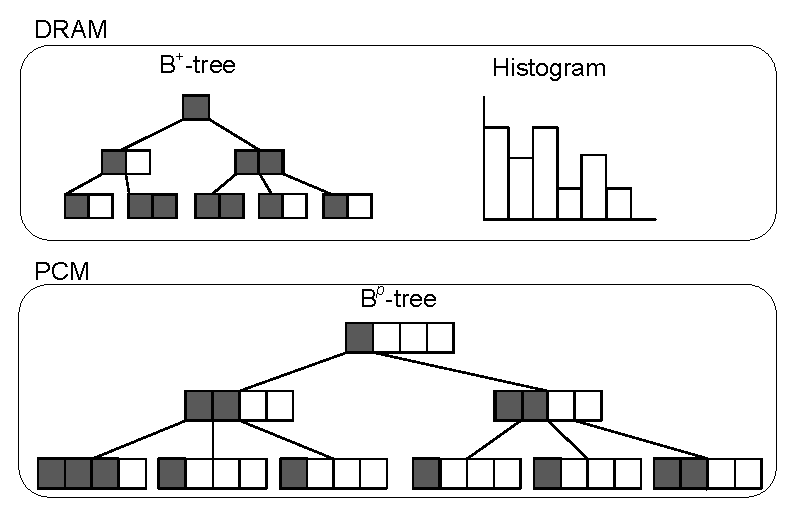
\includegraphics[scale=0.75]{figs/archi.eps}
\caption{\bptree architecture}
\label{fig:archi}
\end{figure}





%For simplicity, we assume \bptree a unique index, that is, there is exactly one record for each key value.
%\bptree is different, such that
%Details of the merge algorithm will be given in Section \ref{sec:algorithm}.
%Since our main idea relies on the prediction, we describe the detail of the prediction model in Section~\ref{sec:prediction}. After that, we describe the basic algorithms of the \bptree.
%\reminder{Add a figure of the architecture} A \bplustree in \pcm, a \bplustree in DRAM, a prediction model



\section{Main Components of {\large \bptree}}
\label{sec:algorithm}

In this section,
we will describe the details of the construction process
of a \bptree.
It consists of two phases, namely the warm-up phase and update phase,
which will be described in Section \ref{sec:warmup}
and Section \ref{sec:build} respectively.


For ease of presentation,
we summarize the notations used throughout this paper in Table~\ref{tab:notations}.

\begin{table}[!t]
\centering \caption{Notations}
\begin{tabular}{|l|p{6.5cm}|} \hline
Parameter&Description \\ \hline \hline
$h$&Height of the \bptree and \bplustree \\ \hline
$2M$&The branching factor of the \bptree on \pcm \\ \hline
$2m$&The branching factor of the \bplustree on DRAM \\ \hline
%$N$&Total number of entries of \bplustree \\ \hline
%$T$&Total number of entries of \bptree \\ \hline
$K$ & $M$ divided by $m$ ($K$ is an integer and $K \ge 1$)\\ \hline
%$b$ & The number of keys in a \bptree node \\ \hline
%$L_i$&Level $i(0\leq i \leq h$) of the tree \\ \hline
%$T_i$&Splitting threshold value of level i($0\leq i \leq h$) \\ \hline
%count$_L$&Number of entries localized in the extent of node L according to the \predict model \\ \hline
%frac$_L$&count$_L$ divided by N   \\ \hline
%$num_{bucket}$&Number of buckets in the histogram \\ \hline$bucket_i$($0$$\leq$$ i $$\leq$$ num_{bucket}$)
$B_i$ & The $i$-th bucket \\ \hline
$n_i$&Number of entries in the $i$-th bucket \\ \hline
\end{tabular}
\label{tab:notations}
\end{table}


\subsection{DRAM Buffer}

As new keys are inserted into the the DRAM buffer continuously,
a small standard \bplustree with branching factor
\emph{2m} is built in the DRAM buffer.
If the buffer is full,
we will flush the keys in the \bplustree to the \bptree on the \pcm.

To capture the data distribution,
we also maintain a histogram.
Suppose the range of the keys is $[L, U]$.
If we want to partition the keys into buckets $B_1, B_2, \cdots, B_{|B|}$,
the bucket width is $\frac{U-L}{|B|}$.
For each bucket $B_i$, we maintain the number of keys that fall in this bucket, denoted by $n_i$.
We will use the histogram to ``forecast'' the data distribution (Section~\ref{sec:model:warm}).

%%%%% lgl:start
%The DRAM buffer offers the following two advantages.
%Firstly, we can update the data in a batch manner onto the \pcm,
%%%% ooibc: check above
%%%% lgl: checked and modified
%which can reduce the number of writes.
%Secondly, we can get more accurate data distribution.
The main function of DRAM buffer is to adaptively adjust our predictive model based on the currently inserted keys in a time window. Then we can use the updated predictive model to merge all the keys in the time window in the \bplustree to the \bptree on \pcm.

%%%%% lgl:end



\subsection{Warm-up Phase} \label{sec:warmup}

Initially, the \bptree on \pcm is empty.
We use a DRAM buffer for warm-up.
We create a standard \bplustree for supporting insertions,
deletions and search.
Before the buffer is full, we use the conventional \bplustree for the initial operations.
For the first time that the DRAM buffer is full,
all the keys in the buffer will be moved to the \pcm,
and this step is called the warm-up process.
The main function of the warm-up phase is to
construct the skeleton of the \bptree on \pcm.

Suppose the DRAM buffer can accommodate $N$ keys.
We first predict the total number of possible keys.
Then, for each \bplustree node,
we use our \predict model to decide whether to split it
in an eager manner to avoid writes for subsequent insertions.
We will provide the details for constructing the initial \bptree
in Section~\ref{sec:model:warm}.


\begin{figure}[!t]
\centering
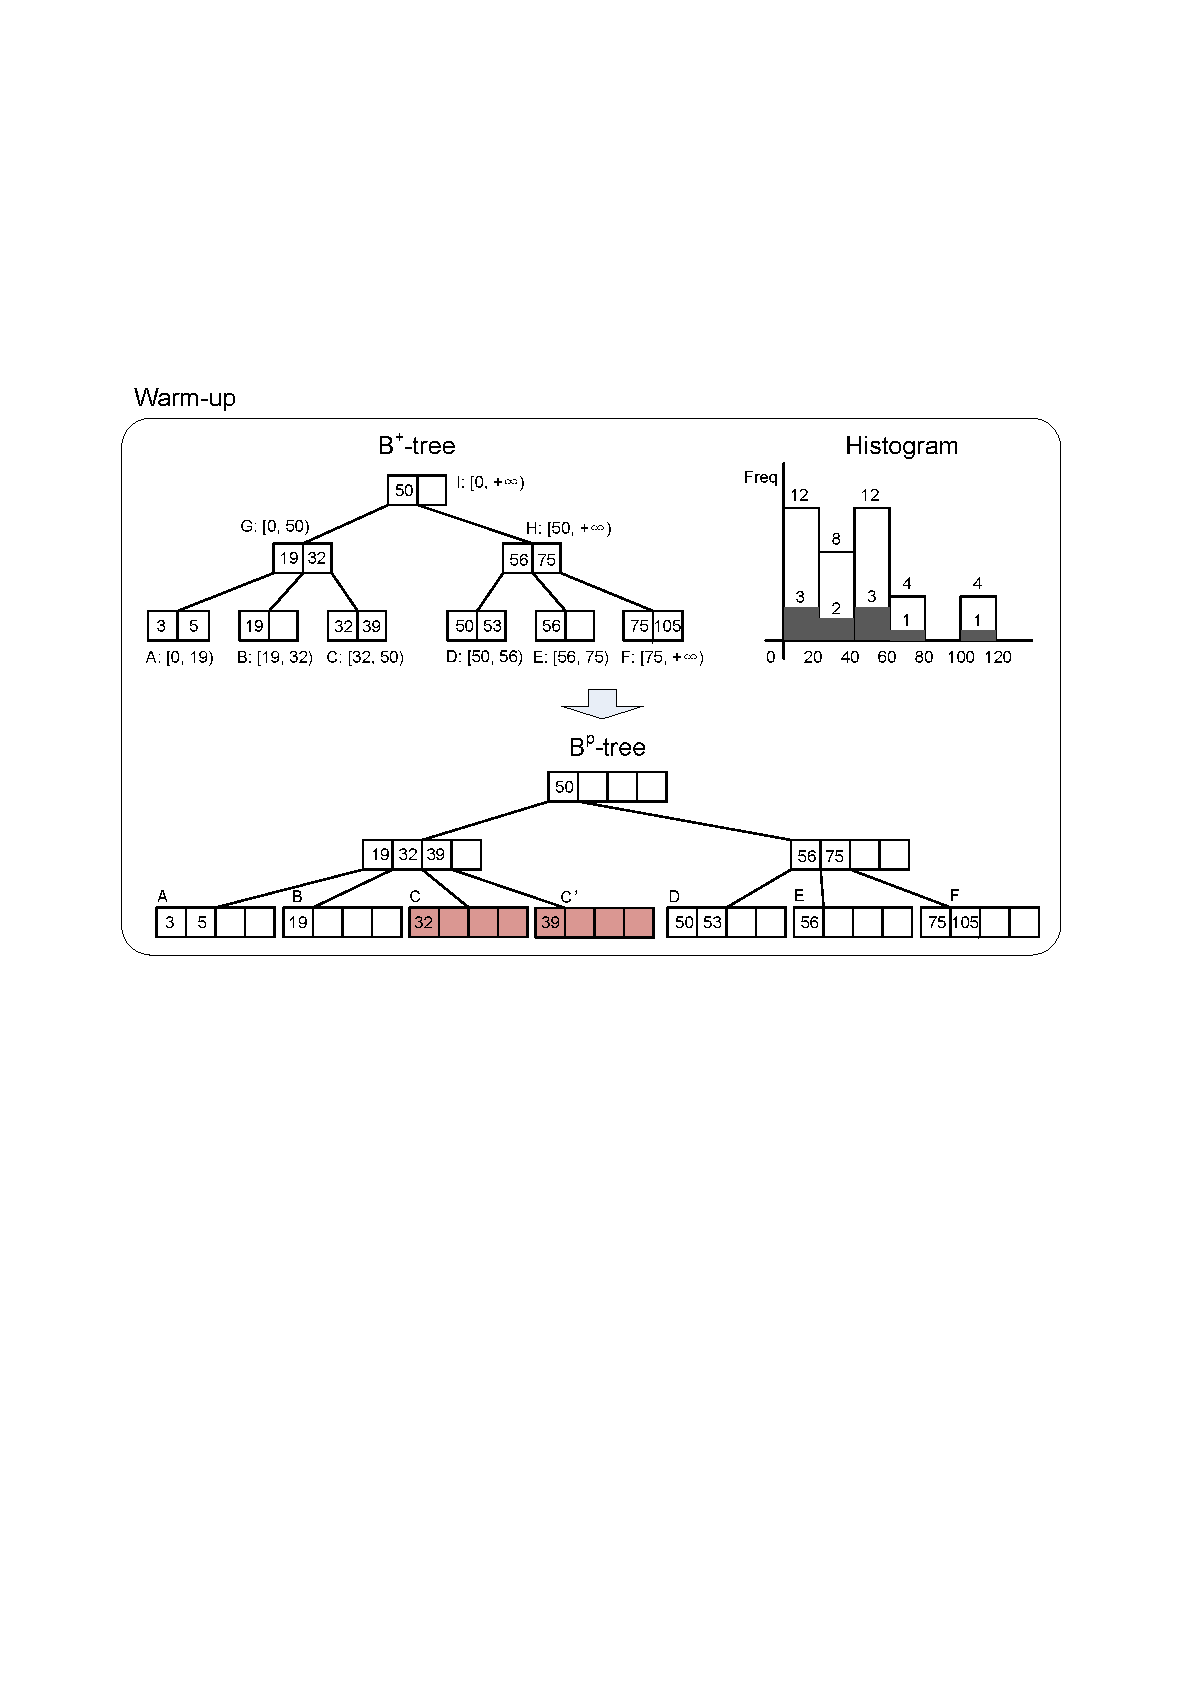
\includegraphics[scale=0.85]{figs/warmup.eps}
\caption{An example of a warm-up phase}
\label{fig:ex:warmup}
\end{figure}

Figure~\ref{fig:ex:warmup} shows an
example for the warm-up phase.
The \bplustree and histogram are in the DRAM and \bptree is in the \pcm.
In this example,
$N$ is 10 and the buffer is full and
thus we need to flush all the keys in the \bplustree to the \pcm.
The black portion of the histogram bar indicates the
number of inserted keys in each range so far, while
the whole bar indicates the predicted number of keys in each range
based on our \predict model.
From this figure,
we can observe that the structure of the \bptree is similar
to that of the original \bplustree.
However, there are two key distinctions.
First, the node could be split in an early manner
if it meets the requirement of node splits.
Second, some of the nodes could \emph{underflow}
due to either an enlargement of the node size or an early split.
These are guided by our \predict model and tree construction strategy.
In the example,
node $C$ in the B$^+$-tree is split into node $C$
and node $C'$ when it is moved to the \bptree,
nodes $B$ and $E$ underflow because of the enlargement of the node size,
while node $C$ and node $C'$ underflow because of the early split.
Details about the early split algorithm
will be presented in Section \ref{sec:model:warm}.

%and generate two nodes and  flush a key $k$ in \bplustree to
%The relative position of all keys in the tree will remain unchanged. We just need to enlarge the size of the tree node and copy all the keys and pointers in each node to the corresponding larger node on \pcm. At this time, the tree on the \pcm is quite sparse and empty, which we call stand of the \bptree.
%Here, \emph{M} is \emph{K} times greater than \emph{m}, that is, . \emph{K} is a parameter of \bptree and needs to be determined in advance.
% In \cite{hankins2003effect}, it has been proved that B$^+$-Tree with node size

%until the buffer is full. firstly insert into the buffer and build a small normal \bplustree. This is because we use it to facilitate the search query. We also need to update the histogram. When the buffer is full, the new \bplustree will be merged into the main \bptree on \pcm. We call each time the merge happens a \emph{time window}.




\subsection{Update Phase}\label{sec:build}

After the warm-up phase,
we have a \bptree structure on the \pcm.
Then for new operations,
we use both the DRAM buffer and
\bptree to handle the operations.
For an insertion, we insert it into the \bplustree.
%%%%% lgl:start
For a search query,
we search the key from both the \bplustree on DRAM and the \bptree on PCM.
If we find it, we return the answer; otherwise we return ``\emptyrst''. (Section~\ref{sec:model:update:search}).
%%%% ooibc: you need to search both regardless of what, as the DRAM buffered tree is a delayed insertion
%%%%  and there may already exist some similar keys in the bptree
%%%%  unless the keys are primary keys, but we do not make such assumptions here
For delete, we search it from both the \bplustree and the \bptree.
If we find it, we remove it from the \bplustree and the \bptree (Section~\ref{sec:model:update:deletion}).
%% TANKL: B+-tree don't need to remove key from non-leaf nodes!!
%The deletion operation on the \bptree has two differences from that on the standard \bplustree. First, we only remove the key from the leaf nodes and do not remove it from internal nodes. Second,
However, even if a node ``underflows'' after deletions, we do not merge it with its siblings. The reason is that since the read latency of PCM is much less
than the write latency, the overhead caused by empty nodes during
query processing is negligible. Furthermore, space could be reserved
for future insertion keys to reduce subsequent writes.
%%%% ooibc: same problem here
For update operation, like other indexes, we treat it as a deletion operation followed by an insertion.
The deletion operation does not need to be buffered, while the following insertion needs to be buffered first like the standard insertion operation on the \bptree.
%The reason we keep a small \bplustree in buffer is to facilitate the search query.
%%%% ooibc: this is not clear -- bigger buffer is better, but we do not have
%%%%       that much memory
Note that we need to update the histogram for the insertion and deletion operations.
If the DRAM buffer is full, we need to merge the \bplustree into the \bptree (Section~\ref{sec:model:update:insertion}).
%%%%% lgl:end


\begin{figure}[!t]
\centering
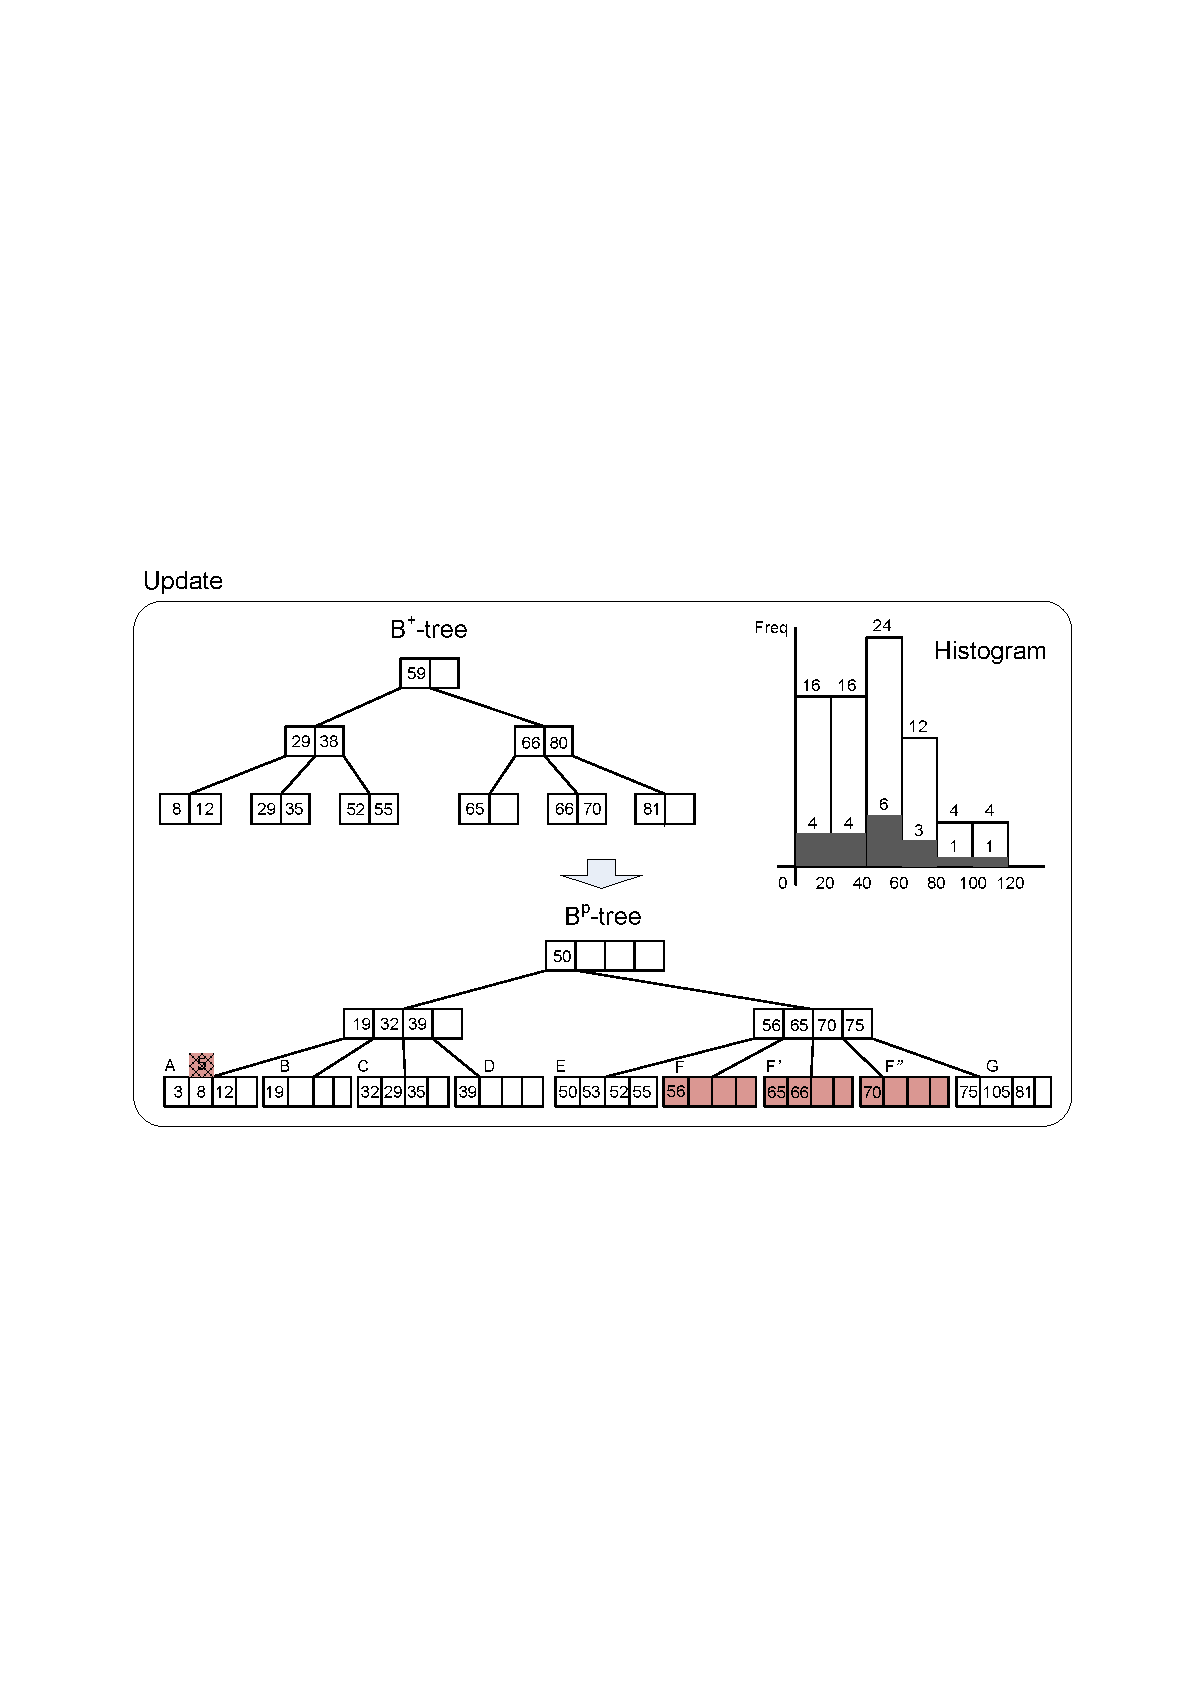
\includegraphics[scale=0.85]{figs/update.eps}
\caption{An example for update phase}
\label{fig:ex:update}
\end{figure}

Figure \ref{fig:ex:update} shows an example for update phase
affected on the earlier example described in Figure~\ref{fig:ex:warmup}.
The case in Figure~\ref{fig:ex:update} is that the buffer is
full for the second time and all the keys in the \bplustree are
merged into the \bptree described in Figure~\ref{fig:ex:warmup}.
In this example for the update phase,
we want to delete the key 5 in the \bptree index from Figure~\ref{fig:ex:warmup}.
First, we search the \bplustree in the buffer and cannot find it.
Then we search the \bptree on the
\pcm and find it in node $A$ and
subsequently remove it from the \bptree.
As can be seen from the figure,
the histogram is updated to reflect the effect of this deletion
and the new round of prediction is performed based on all the keys inserted
currently including the keys in the buffer.
Node $F$ in the \bptree is split because of the similar
reason as that of the node C in Figure~\ref{fig:ex:warmup}.
We will describe the details in Section~\ref{sec:model:update}.

\section{Summary}

In this chapter, we introduced our \bptree. We present the design principle and basic idea of \bptree. 
We know that there are two major parts of \bptree including the DRAM buffer and the normal \bplustree on \pcm. 
When new keys are inserted into the \bptree, there are two phases. First, the new key is inserted into 
the small \bplustree on the DRAM buffer, when the DRAM buffer is full for the first time, we merge the 
whole tree to \pcm and construct the skeleton of the tree on \pcm based on the predictive model. After 
that each time when the DRAM is full, we will merge the tree to the existing \bplustree on \pcm. 
During the construction, the node of our \bptree may be ``underflow'' which is different from the traditional
\bplustree. The reason is that sometimes we want to split the node in advance based on the prediction model even
the node is not full. In our design, even some nodes may be ``underflow'', we will still use some strategy to 
ensure that the whole tree is in a good shape. We will talk about the details about the prediction model 
and the construction process in next chapter. 

\newpage
